%\documentclass[reponses, utf8, 11pt]{feuille}
\documentclass[utf8, 11pt]{feuille}

\newcommand{\titredutd}{\textbf{TD8 --- L'ensemble canonique~: capacité calorifique}}

\begin{document}


\begin{tcolorbox}[
        colback=gray!20,
        colframe=gray!20,
        width=\dimexpr\textwidth\relax, 
        arc=0pt,outer arc=0pt,
        ]

\texttt{Seules les calculatrices non communicantes et les notes manuscrites personnelles sont autorisées.}

\texttt{Les exercices sont totalement indépendants.}

\texttt{On notera $k_B$ la constante de Boltzmann et $h$ la constante de Planck.}

\end{tcolorbox}



% ______________________________________________________________________________
\section{\soft~Étude du paramagnétisme}

Un cristal paramagnétique est formé de $N$ atomes portant chacun un moment magnétique $\overrightarrow{\mu}$. Le système, en contact avec un thermostat à la température $T$, est plongé dans un champ magnétique $\overrightarrow{B}$ orienté selon l'axe $Oz$.  On rappelle que l'énergie potentielle d'un moment magnétique $\overrightarrow{\mu}$ dans un champ $\overrightarrow{B}$ est $e=-\overrightarrow{\mu}.\overrightarrow{B}$ et on néglige les interactions entre les moments magnétiques.

\medskip

{\sffamily\bfseries{Description classique}}

Chaque moment magnétique $\overrightarrow{\mu}$ a une norme fixe $\mu$ et peut s'orienter dans une direction quelconque, repérée par les angles $\theta$ et $\phi$ des coordonnées sphériques. Un moment magnétique étant assimilé à un rotateur de moment d'inertie $\cal I$, son hamiltonien est donné par
$$
h=\frac{p_{\theta}^2}{2 {\cal I}} + \frac{p_{\phi}^2}{2 {\cal I}\sin^{2} \theta} -\mu B \cos \theta
$$

\question
Exprimer la fonction de partition $Z$ du système à l'aide de la fonction de partition $z$ d'un seul moment magnétique. Montrer que $z$ s'exprime sous la forme $z=z_{cin}z_{mag}$ où $z_{mag}$ s'exprime en fonction de $x=\beta \mu B$ et vaut 1 pour $x=0$ . Montrer que $z_{cin}$ est de la forme $z_{cin}=\frac{\cal V}{\Lambda_T^2}$ où $\cal V$ est un \og volume accessible\fg, et $\Lambda_T$ une longueur  thermique.

\question
Calculer l'énergie moyenne $\langle E \rangle$. Quelle est la contribution moyenne de l'énergie cinétique $\langle E_{\rm cin} \rangle$ ? En déduire la valeur moyenne $\langle E_{\rm mag}\rangle $ de l'énergie d'interaction avec le champ magnétique.

\question
Donner la densité de probabilité $P(\theta, \phi)$ qu'un moment magnétique pointe dans la direction donnée par les angles $\theta$ et $\phi$ à ${\rm d}\theta$ et ${\rm d}\phi$ près. Vérifier qu'en l'absence de champ magnétique la distribution de probabilité est bien isotrope. On rappelle que l'élément d'angle solide est ${\rm d}^2 \Omega= \sin \theta {\rm d} \theta {\rm d} \phi$.

\question
Calculer les valeurs moyennes $\langle \mu_x \rangle$, $\langle \mu_y \rangle$ et $\langle \mu_z \rangle$ des projections de $\overrightarrow{\mu}$ selon les axes $Ox, Oy$ et $Oz$. On exprimera $\langle \mu_z \rangle$ à l'aide de la fonction de Langevin définie par
$$
{\cal L}(x)=\frac{1}{\tanh x}-\frac{1}{x}\enspace.
$$
Tracer l'aimantation moyenne $\langle M \rangle$ en fonction de $x$.

\medskip

{\sffamily\bfseries{Description quantique : modèle de Brillouin}}

Dans le cas général, le spin porté par les atomes du cristal est un
entier ou un demi-entier $J$. La projection du moment magnétique selon
l'axe $z$ peut prendre alors $2J+1$ valeurs : $\mu_z= -g\mu_B J_z$, où
$g \simeq 2$ est le facteur de Landé et $\mu_B$ le magnéton de Bohr,
avec $J_z=-J, -J+1, \dots,J-1, J$.

\question
Calculer la fonction de partition $z$ d'un spin. On posera $x= \beta g \mu_B B$.

\noindent
On rappelle que pour une série géométrique de raison $q$ : $\displaystyle S_N=\sum_{n=0}^{N} q^n=\frac{1-q^{N+1}}{1-q}$.  

\question
En déduire la valeur moyenne $\langle \mu_z \rangle$ du moment magnétique, que l'on exprimera à l'aide de la fonction de Brillouin d'ordre $J$ donnée par
$$
{\cal B}_J(y)=\frac{2J+1}{2J} \coth \Big[\frac{2J+1}{2J}y\Big]-\frac{1}{2J}\coth \Big(\frac{y}{2J}\Big)\enspace.
$$

\question
Dans le cas particulier où $J=1/2$ et en posant $\mu = g\mu_B J$, que devient l'expression de $\langle \mu_z \rangle$. Commenter ce résultat. 

\question
On donne au voisinage de l'origine  ${\cal B}_J(y)= \frac{J+1}{3J} y+O(y^3)$. Montrer qu'à haute température, on retrouve à nouveau la loi de Curie, mais qu'à faible température, on est loin du résultat classique obtenu dans la partie précédente (sauf dans la limite des grandes valeurs de $J$).

\begin{figure}[h]
\begin{center} 
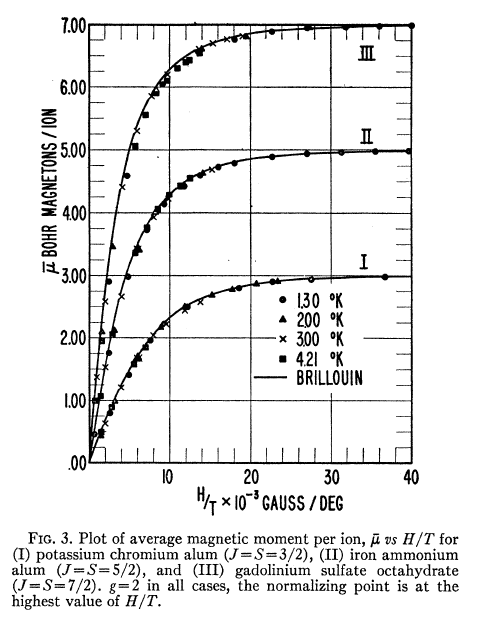
\includegraphics[height=.5\textwidth]{brillouin}
\caption{\it Moment magnétique moyen par ion (en unité du magnéton de Bohr) en fonction de $B/T$ pour certains sels paramagnétiques : (I) Cr$^{3+}$, (II) Fe$^{3+}$ et (III) Gd$^{3+}$.  Les points sont les données expérimentales et les courbes en traits pleins correspondent aux résultats obtenus en utilisant des fonctions de Brillouin [tirée de W. E. Henry, Phys. Rev. \textbf{88}, 559 (1952)]. Pourriez vous estimer la valeur de $J$ pour chaque ion ?}
\end{center} 
\end{figure}



\elements{\\
1 : $z_{cin} = \frac{8 {\cal I} \pi^2}{\beta h^2}$, $z_{mag} = \left( \frac{\sinh(\beta \mu B)}{\beta \mu B} \right) $. Volume accessible ${\cal V} = \frac{4 {\cal I} \pi}{m}$, et $\Lambda_T$ longueur thermique de de Broglie.
\\
2 : $\langle E \rangle = N \langle e \rangle$ et $\langle e_{cin} \rangle = k_B T$, $\langle e_{mag} \rangle = k_B T - \mu B \coth(\beta \mu B)$.
\\
3 : $P(\theta, \phi) = \frac{1}{4 \pi} \frac{\beta \mu B}{\sinh(\beta \mu B)} \sin \theta e^{\beta \mu B \cos \theta}$.
\\
4 : $\langle \mu_x \rangle = \langle \mu_y \rangle = 0$ et $\langle \mu_z \rangle = \mu {\cal L} (\beta \mu B)$.
\\
5 : $z = \frac{\sinh(x(J+\frac{1}{2}))}{\sinh(\frac{x}{2})}$.
\\
6 : $\langle u_z \rangle = g \mu_B J {\cal B}_J(\beta g \mu_B B J)$.
\\
7 : ${\cal B}_J(y) = \tanh(y)$, et $\langle \mu_z \rangle = \mu \tanh( \beta \mu B)$ : résultat classique obtenu pour un système à 2 niveaux.
\\
8 : La loi de Curie énonce que la susceptibilité d'un matériaux pramagnétique est en $\frac{1}{T}$. Or $\chi_m = \mu_0 \partial_B M$ avec l'aimantation $M = n_v \langle \mu \rangle$ où $n_v$ est la densité volumique de moments magnétiques. Le calcul de $\chi_m$ donne la constante de Curie $\farc{\mu_0}{3} n_v (g \mu_B)^2 \frac{J(J+1)}{B}$. La pente à l'origine sur la Fig. est $\chi_m$, d'où la valeur de $J$.
}



% ______________________________________________________________________________
\section{\medium~Capacité calorifique des gaz diatomiques}

On se propose de déterminer l'expression de la capacité calorifique d'un gaz de molécules diatomiques  hétéro-nucléaires (avec deux atomes différents). On admet que l'Hamiltonien d'une telle molécule diatomique peut s'écrire sous la forme de trois termes principaux $h = h_{tr} + h_{rot} + h_{vib}$. On a respectivement

\begin{itemize}

\item 
$h_{tr} =\frac{\vec{P}^2}{2M}$ où $\vec{P}$ est la quantité de mouvement de la molécule et $M$ sa masse

\item
$h_{rot} =\frac{\vec{l}^2}{2I}$ où $\vec{l}$ est le moment cinétique orbital caractérisant la rotation de la molécule et $I$ le moment d'inertie correspondant (par rapport à  un axe passant par le centre de gravité de la molécule et perpendiculaire à  l'axe rejoignant les deux atomes)

\item
$h_{vib} =\frac{p_x^2}{2\mu}+\frac{k x^2}{2}$, hamiltonien d'un oscillateur harmonique à  une dimension ($x$ est l'écart à  la distance d'équilibre entre les deux molécules et $p_x$ l'impulsion correspondante; $\mu$ est ici la masse réduite des deux atomes).

\end{itemize}


Les valeurs propres de cet Hamiltonien, dans l'approximation du découplage entre ces différentes formes d'énergie, sont telles que l'énergie de la molécule s'écrit $\epsilon =\epsilon_{tr}+\epsilon_{rot}+\epsilon_{vib}$.

On considère un gaz très dilué de $N$ molécules diatomiques identiques à  la température $T$ dans le volume $V$. On suppose que la fonction de partition totale $Z=Z(N,V,T)$ peut s'écrire $Z= z^N/N!$ où $z=z(V,T)$ est la fonction de partition correspondant à  une seule molécule.

\question{Donner trois exemples de gaz diatomiques hétéro-nucléaires.}

\question{Préciser le sens physique de la factorisation $Z= z^N/N!$.}

\question{Rappeler dans l'ensemble canonique la relation entre $Z$ et l'énergie moyenne $\langle E \rangle$ du système. En déduire que la capacité calorifique à  volume constant $C_V$ est donnée par $\frac{C_V}{k_B}=\beta^2 \left( \frac{\partial^2 \ln Z}{\partial \beta^2} \right)_V$.} 

\question{Montrer que, dans les conditions de l'énoncé, $z$ peut s'écrire $z=z_{tr}z_{rot}z_{vib}$ en explicitant le sens de chaque terme. En déduire que l'énergie moyenne et  la capacité calorifique du gaz peuvent s'écrire sous la forme de sommes de trois termes,
associés aux trois différentes formes de l'énergie.}

\question{Combien de degrés de liberté quadratiques possède cette molécule ? En utilisant le théorème d'équipartition que l'on énoncera, que prédit-on dans la limite classique pour l'énergie moyenne et la capacité calorifique par molécule ?}


{\sffamily\bfseries{L'énergie cinétique de translation}}

Aux températures considérées, on peut effectuer un calcul classique pour estimer $z_{tr}$.

\question{Donner sous forme intégrale l'expression de $z_{tr}$. On introduira $h$ la constante de Planck.}

\question{On rappelle que $\int_{-\infty}^{+\infty} \D u \exp(-u^2)=\sqrt{\pi}$. Montrer que $z_{tr}=\frac{V}{\Lambda^3}$ où $\Lambda$ est une grandeur que l'on déterminera en fonction de $M$, $h$ et $k_BT$.}

\question{En déduire l'énergie moyenne $e_{tr}$ par molécule et la capacité calorifique (à  volume constant) correspondante $c_{tr}$. Comment cette dernière dépend-t-elle de la température ?}


{\sffamily\bfseries{L'énergie de vibration}}

\question{Rappeler l'expression des différents niveaux d'énergie discrets d'un oscillateur harmonique quantique à  une dimension. L'énergie du niveau fondamental est $\frac{\hbar \omega}{2}$ et on introduit la température de vibration associée $\Theta_{\mathrm{vib}} = \frac{\hbar \omega}{2 k_B}$.}

\question{Montrer que $z_{vib}=\frac{1}{2 \sinh(\frac{\hbar \omega}{2 k_B T})}$.}

\question{En déduire l'énergie moyenne $e_{vib}$ par molécule et la capacité calorifique (à  volume constant) correspondante $c_{vib}$. Comment cette dernière dépend-t-elle de la température ? On pourra étudier les limites basses températures et hautes températures.}


{\sffamily\bfseries{L'énergie de rotation}}

Les niveaux d'énergie d'une molécule di-atomique en rotation considérée comme un rotateur rigide sont donnés
par l'expression $\epsilon_{rot}=\frac{\hbar^2}{2I}J(J+1)$ où $0 \le J \le + \infty$ est le nombre quantique (entier) de rotation. Il y a $2J+1$ états dégénérés pour cette valeur de $J$. Il est utile d'introduire la température caractéristique $\theta_{\mathrm{rot}}=\hbar^2/(2Ik_B)$ et le rapport $x =\frac{\theta_{\mathrm{rot}}}{T}$ pour alléger les notations.

\question{\'Ecrire l'expression de la fonction de partition $z_{rot}$ (sans la calculer).}

\question{Dans la limite haute température, on peut développer $z_{rot}$ sous la forme $z_{rot}=\frac{1}{x} \left( 1+\frac{x}{3}+\frac{x^2}{15}+\ldots \right)$. En déduire l'énergie moyenne $e_{rot}$ par molécule et la capacité calorifique (à  volume constant) correspondante $c_{rot}$ dans cette limite. Montrer alors que $c_{rot}$ décroît avec la température.}

\question{Dans la limite basse température, seuls les niveaux de basse énergie seront peuplés. Montrer en conservant le nombre de termes adéquats dans la fonction de partition que, dans cette limite, $c_{rot}=12 k_B x^2 \exp(-2x)$.}

\question{En déduire l'allure probable de $\frac{c_{rot}}{k_B}$ en fonction de $\frac{T}{\theta}$.}

\question{Déduire de toutes les questions précédentes l'expression de la capacité calorifique à  volume constant ${\cal C}_V$ dans la limite haute température.}



\subsection{Application au HD}

Le deutérure d'hydrogène est formé d'un proton H et d'un atome de deutérium D. On a dans ce cas $\theta_{\mathrm{rot}}=64$ K et $\frac{\hbar \omega}{k_B}=5382$ K. Calculer ${\cal C}_V$ à  l'ambiante (300 K) et à  3000 K.

%\section{Une condensation à  deux dimensions ?}
%On considère un modèle de fluide  à  deux dimensions, surface $S$, température $T$ et potentiel chimique $\mu$ comme un \og gaz \fg \ de bosons  indépendants de spin nul, de masse $m$ et dont les niveaux d'énergie  sont donnés par
%\begin{align*}
%\epsilon (k)=\frac{\hbar^2 k^2}{2m},
%\end{align*}
%où $k$ est le vecteur d'onde.
%
%\question{Rappeler l'expression du nombre moyen d'occupation $n(\epsilon)$ d'un micro-état d'énergie $\epsilon$.}
%
%\question{Montrer que la densité en énergie des micro-états s'écrit sous la forme $\rho (\epsilon)=A$ où le calcul de $A$ fait appel à  la quantification du vecteur d'onde dans la boîte de surface $S=L_xL_y$. On utilisera des conditions aux limites périodiques pour exprimer les valeurs autorisées de $\vec{k}$.}
%
%\question{En déduire les expressions formelles du nombre moyen $\langle N \rangle$ de particules et de leur énergie moyenne $\langle E \rangle$ sous forme intégrale, en fonction de $T, S$ et $\mu$ et des données. On introduira $\alpha=N\frac{\Lambda^2}{S}$ où $\Lambda=\frac{h}{\sqrt{2\pi m k_B T}}$. }
%
%\question{On donne l'intégrale $\int_0^{+\infty} \frac{dx}{e^{x-y}-1}=-\ln \left(1-e^y \right)$. Calculer explicitement $\mu $ en fonction de $k_BT$ et de $\alpha$.}
%
%\question{En déduire que, dans le cas d'un fluide de bosons bidimensionnel, il n'y a pas de condensation de Bose-Einstein.}




\end{document}
